\documentclass[
	paper=A4,
	twoside=false,
	parskip=full,
	chapterprefix=true,  
	appendixprefix=true,
	12pt,
	headings=normal,
	bibliography=totoc,
	titlepage=on,
	draft=false,
]{scrreprt}
\usepackage{setspace}
\usepackage{booktabs}
\usepackage{tabularx}
\usepackage[utf8]{inputenc}
\usepackage[T1]{fontenc}
\usepackage[french]{babel}
\usepackage[
	sansserif=false,
	colorize=full,
	hangsection,
	hangsubsection, 
	hangfigurecaption=false,
	colorize=full,
	colortheme=bluemagenta,
	bibsys=bibtex,
	bibfile=main,
	bibstyle=numeric,
]{cleanthesis} 
   
\usepackage{pdfpages}
\usepackage{hyperref}
\usepackage{tikz} 
\usepackage{amsmath}
\usepackage{amsfonts}
\usepackage{amssymb}
\usepackage{amsthm}
\usepackage{amsbsy}
\usepackage{biblatex}
\usepackage{makeidx}
\usepackage{framed}
\usepackage{float}
\usepackage[acronym]{glossaries}
\usepackage{listings}
\usepackage{booktabs}
\usepackage[toc,page]{appendix}
\usepackage[mode=buildnew]{standalone}
\usepackage{xparse}
\usepackage[printonlyused,withpage]{acronym}
\usepackage{graphicx}

% titelseite info
\newcommand{\Cs}{C\#}
\newcommand*{\quelle}{% 
  \footnotesize Quelle: 
} 
\graphicspath{ {img/} }
\newcommand{\norm}[1]{\left\lVert#1\right\rVert}
\newcommand{\Autor}{}
\newcommand{\MatrikelNummer}{32}
\newcommand{\Kursbezeichnung}{L2 S4 Automne}
\newcommand{\Was}{Rendu de projet}
\newcommand{\Titel}{Rendu de projet}
\newcommand{\AbgabeDatum}{13 décembre 2020}

\includeonly{
 %erklaerung
 ,abstract
 ,trie
 ,dawg
 ,application
 ,test
 ,analyse
 ,conclusion
 %,kapitel1
 %,kapitel2
 %,einleitung
 %,technologien
 %,umsetzung
 %,deployment
}

% JavaScript

\definecolor{lightgray}{rgb}{.9,.9,.9}
\definecolor{darkgray}{rgb}{.4,.4,.4}
\definecolor{purple}{rgb}{0.65, 0.12, 0.82}

\lstdefinelanguage{JavaScript}{
  morekeywords=[1]{break, continue, delete, else, for, function, if, in,
    new, return, this, typeof, var, void, while, with},
  % Literals, primitive types, and reference types.
  morekeywords=[2]{false, null, true, boolean, number, undefined,
    Array, Boolean, Date, Math, Number, String, Object},
  % Built-ins.
  morekeywords=[3]{eval, parseInt, parseFloat, escape, unescape},
  sensitive,
  morecomment=[s]{/*}{*/},
  morecomment=[l]//,
  morecomment=[s]{/**}{*/}, % JavaDoc style comments
  morestring=[b]',
  morestring=[b]"
}[keywords, comments, strings]

\lstdefinelanguage{JSON}{
    string=[s]{"}{"},
    stringstyle=\color{blue},
    comment=[l]{:},
    commentstyle=\color{black},
}

% For inputting other files
\newcommand\inputfile[1]{%
    \InputIfFileExists{#1}{}{\typeout{No file #1.}}%
}
 
% Nicht zitierte Quellen, die trotzdem in der Bibliographie auftauchen sollen
\nocite{*}

%lsiting optionen
\lstset{language=[Sharp]C,numbers=left,numberstyle=\tiny,breaklines,tabsize=4}
 
\lstset{literate=
  {Ö}{{\"O}}1
  {Ä}{{\"A}}1
  {Ü}{{\"U}}1
  {ß}{{\ss}}1
  {ü}{{\"u}}1
  {ä}{{\"a}}1
  {ö}{{\"o}}1
}

% --------------
%  Front Matter
% --------------

\pagenumbering{roman}
\pagestyle{empty}

\begin{document}

%%%%%%%%%%%%%%%%%%%%%%%Titelseite%%%%%%%%%%%%%%%%%%%%%%%%%%%%%%%%%%%%%%%%%%%%%%%%%%%

\begin{titlepage}
    \begin{center}
        \vspace*{2.5cm}
        %\FirmenLogoDeckblatt\hfill\includegraphics[width=4cm]{img/dhbw-logo}\\[2cm]
        %{\Huge \Titel}\\[2cm]
        {\Huge\scshape \Was}\\[1.5cm]
        {\large « Détection automatique de langue »}\\[1cm]
        {\large SDA2 }\\[1cm]
        %{\large des Studienganges \Studiengang}\\[0.5cm]
        %{\large an der}\\[0.5cm]
        {\large UFR Math-Info - Université de Strasbourg}\\[0.5cm]
        {\large 2\textsuperscript{ième} année de Licence Informatique}\\[1cm]
        %{\large\bfseries \Autor}\\[1cm]
        {\large Date de rendu: \AbgabeDatum}\\[2cm]
        {\large Par}\\[0.5cm]
        {\large Matthieu FREITAG}\\[0.15cm]
        {\large et Paul MEYER}\\[4cm]
        {\large \href{https://github.com/Zapharaos/ProjetSDA2}{https://github.com/Zapharaos/ProjetSDA2}}
        \vfill
    \end{center}
\end{titlepage}
\clearpage

\pagestyle{plain}
%%%%%%%%%%%%%%%%%%%%%%%%%%%%%%%%%%%%%%%%%%%%%%%%%%%%%%%%%%%%%%%%%%%%%%%%%%%%%%%%%%%%

% Verzeichnisse
\setcounter{tocdepth}{1}

% include abstract
\pdfbookmark[0]{Abstract}{Abstract}
\chapter*{Problème}
\label{sec:abstract}
\vspace*{-10mm}

On se propose d’étudier dans ce projet une méthode de détection automatique d’une langue.
Pour simplifier cette étude, seuls l’allemand, l’anglais ainsi que le français seront considérés. Les
accents et la ponctuation que l’on peut retrouver dans la langue française et allemande ne seront
quant à eux pas utilisés.

\section*{\color{black}Approche proposée}
\begin{enumerate}
\item Analyse des dictionnaires allemand, anglais et français.
\item Lecture du texte à identifier.
\item Pour chaque mot du texte à identifier, tester la correspondance du mot par rapport à
chacun des dictionnaires
\item La langue du texte est celle avec le plus grand nombre de correspondances positives.
\end{enumerate}

\newline Pour ce faire, on nous propose deux structures de données que nous allons devoir implémenter : le trie et le dawg.\newline Ces structures vont contenir les dictionnaires allemand, anglais et français.



\renewcommand\contentsname{\usekomafont{chapter}\mdseries Index} % Ohne diese haben die überschriften der Verzeichnisse die komische komafont-schriftart
\tableofcontents

\printnoidxglossary[type=\acronymtype,title=Abréviations,toctitle=Abréviations] % Abkürzungen
\clearpage 
 
\setglossarystyle{altlist} % Danach Style auf "ausführlichere" Liste umschalten
\printnoidxglossary[nonumberlist] % Glossar, ohne Seitenzahlen für Referenzen
\clearpage

%\lstlistoflistings

%\renewcommand\listfigurename{\usekomafont{chapter}\mdseries Abbildungsverzeichnis}
%\listoffigures

%\renewcommand\listtablename{\usekomafont{chapter}\mdseries Tabellenverzeichnis}
%\listoftables

\clearpage

%\include{abk}

% -------------
%  Body Matter
% -------------

\pagenumbering{arabic}
\setcounter{page}{1}
\pagestyle{maincontentstyle}
 
%\include{einleitung}
\chapter{Arbre préfixe : Trie}

\section{Structure de données}

On se servira d'un tableau de Trie de taille 26 et d'une structure Lang qui stocke trois booléens permettant d'indiquer les langues d'un mot. \bigskip \newline Chaque lettre aura un tableau de 26 successeurs de type Trie avec des booléens permettant d'indiquer si c'est un mot ainsi que ses langues.

Ceci nous permet de réduire la place mémoire en insérant les dictionnaires dans une unique structure Trie. Notamment dans le cas des doublons, on évite de stocker le même mot et on se sert de la structure Lang pour indiquer qu'il existe dans plusieurs langues. Démonstration dans la partie 4 : "Tests".

\section{Insertion}

Pour insérer dans un Trie, on va parcourir un mot récursivement, lettre après lettre. Pour chaque lettre, on regarde si elle est déjà existante dans le tableau, le cas échéant on alloue une case, puis on poursuit l'insertion.
\bigskip \newline L étant la longueur du mot, alors on peut dire qu'en pire cas, il faudra allouer L lettres. Ce qui donne O(L*log(n)) pour un ensemble n de mots.

\section{Recherche}

De la même manière, pour rechercher un mot dans un Trie, on va parcourir un mot récursivement, lettre après lettre, tout en avançant dans le Trie. Si il est impossible de continuer le parcours et que le mot n'a pas été traité totalement, alors on retourne "inconnu". Sinon, on retourne les langues correspondantes.
 \bigskip \newline L étant la longueur du mot, il faudra donc chercher L lettres dans le tableau. Ce qui donne O(L).

\chapter{Directed Acyclic Word Graph : DAWG}

Note : les fonctions d'insertion et de minimisation figurant dans le sujet, nous avons décidé de ne pas les expliquer dans notre rapport.

\section{Les structures de données}

Pour le dawg, nous avons implementé trois structures de données :

Une structure dawg qui contient une structure hashmap, une structure stack et une structure node (i.e la racine). De plus, elle contient le dernier mot inséré et l'ID de sa dernière lettre (i.e. son dernier noeud). 

Une structure node qui contient un ID, un booléen permettant d'indiquer si la lettre est finale et un tableau de 26 edges.

Une structure edge qui contient une lettre ainsi que des pointeurs vers le noeud actuel et le noeud suivant.

\section{Recherche}

De la même manière que dans le Trie, pour rechercher un mot dans un Dawg, on va parcourir un mot récursivement, lettre après lettre, tout en avançant dans le Dawg. Si il est impossible de continuer le parcours et que le mot n’a pas été traité totalement, alors on retourne false. Sinon, on retourne true.


\chapter{Mise en application}

Note : Avant de lancer le programme pour la première fois il est nécessaire d'entrer la commande suivante :
\begin{lstlisting}[language=bash]
    $ make && make dict
\end{lstlisting}

\section{Le mode utilisateur}

Pour lancer le programme en mode utilisateur :
\begin{lstlisting}[language=bash]
    $ ./bin/ald -sentence -trie/dawg
\end{lstlisting}

Le programme chargera les dictionnaires dans le mode demandé puis vous demandera d'entrer une phrase. Il la traitera et vous affichera le résultat. 
\newline Et si vous le souhaitez, vous pouvez entrer une nouvelle phrase.

\section{Les modes tests}

D'autres options existent et permettent d'effectuer des tests :
\begin{lstlisting}[language=bash]
    $ ./bin/ald -test
    $ ./bin/ald -perf -trie/dawg
\end{lstlisting}

Elles seront détaillées dans la section suivante.

\section{Autres}

Si vous avez besoin d'aide, ces commandes peuvent vous guider :
\begin{lstlisting}[language=bash]
    $ ./bin/ald -help
    $ make list
\end{lstlisting}

\chapter{Tests}

Note : Nous utiliserons une structure Trie par langue afin de pouvoir comparer le Trie et le Dawg de manière équitable.

\section{Vérification de l'insertion}

On va compter le nombre de noeuds dans chaque structure Trie et Dawg via un DFS et comparer les valeurs avec celles données dans le sujet. Si elles sont égales, alors les insertions devraient être fonctionnelles.

Voici comment lancer le test :
\begin{lstlisting}[language=bash]
    $ ./bin/ald -count -trie/dawg
\end{lstlisting}

Objectifs dans un Trie
\begin{itemize}
\item Français : 623 994
\item Allemand : 1 229 117
\item Anglais : 606 879
\end{itemize}

Objectifs dans un Dawg
\begin{itemize}
\item Français : 34 202
\item Allemand : 146 205
\item Anglais : 80 075
\end{itemize}

En lançant le programme on remarque que les valeurs sont égales.

De plus, on lance le test avec un Trie contenant les trois dictionnaires et on obtient le nombre de noeud suivant : 2 296 705. \newline Or, le nombre de noeuds de chaque dictionnaire additionné nous donne 2 459 990. On en déduit que notre méthode est plus efficace.

\section{Vérification de la recherche}

Nous utilisons une structure par langue et recherchons le dictionnaire complet de cette langue dans la structure. On comptera le nombre de mots trouvés et il devra correspondre au nombre de mots insérés.

Voici comment lancer le test :
\begin{lstlisting}[language=bash]
    $ ./bin/ald -test
\end{lstlisting}

Objectifs dans un Trie
\begin{itemize}
\item Français : 336 528
\item Allemand : 685 620
\item Anglais : 274 411
\end{itemize}

En lançant le programme on remarque que les valeurs sont égales.

\section{Évaluation des performances}

Commande pour lancer le test de performance :
\begin{lstlisting}[language=bash]
    $ ./bin/ald -perf -trie/dawg
\end{lstlisting}

Pour l'insertion :
\smallskip \newline Nous allons insérer n mots, avec n débutant à 10. Le compteur sera multiplié par 2 après chaque tour et ceci jusqu'à ce qu'il n'y ai plus de mots dans le fichier. Nous effectuerons le test 10 fois pour chaque n.

Pour la recherche :
\smallskip \newline Nous allons lire une ligne aléatoire dans le fichier et rechercher le mot qui s'y trouve.
Cette étape sera effectuée 10 fois pour chaque n, avec n allant de 10 à 20 971 520 (n sera multiplié par 2 après chaque tour).

Nous obtenons des graphiques qui seront étudiés dans la section suivante.
\chapter{Analyse}
\graphicspath{ {./images/} }

\section{Insertion}

\begin{figure}[H]
    \centering
    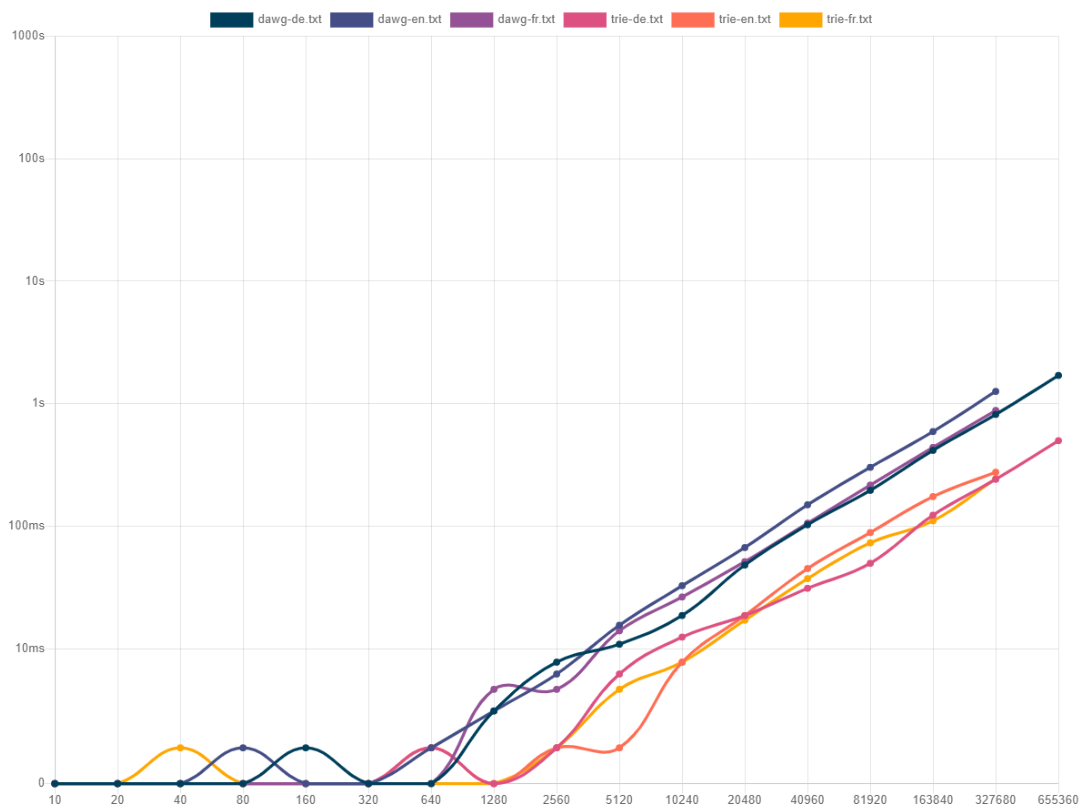
\includegraphics[scale=0.5]{images/time_insert.png}
    \caption{\label{HomePage} Temps d'insertion}
\end{figure}

On rappelle que, en théorie :
\begin{itemize}
  \item[-] Trie : O(L * log(n)) avec L la longueur maximale d'un mot et n le nombre de mots
  \item[-] Dawg : O(log(n)) avec n le nombre d'état dans le dictionnaire.
\end{itemize} \leavevmode

En pratique : \medskip \newline
L'insertion dans les deux structures semble être de même complexité, même si l'insertion dans un Trie prend environ deux fois moins de temps que dans un Dawg.\newline Ce qui est normal car il faut minimiser la structure Dawg à chaque insertion.

\section{Recherche}

\begin{figure}[H]
    \centering
    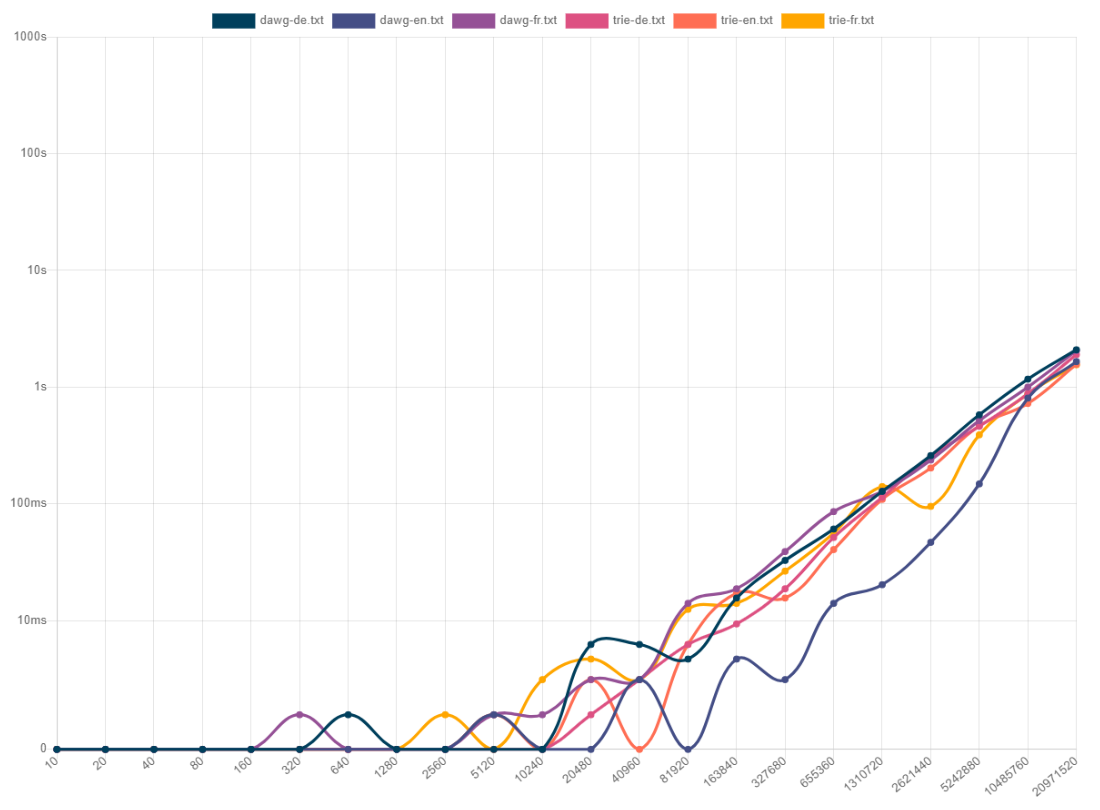
\includegraphics[scale=0.5]{images/time_search.png}
    \caption{\label{HomePage} Temps de recherche}
\end{figure}

On rappelle que, en théorie :
\begin{itemize}
  \item[-] Trie : O(L) avec L la longueur maximale d'un mot.
  \item[-] Dawg : O(log(n)) avec n le nombre d'état dans le dictionnaire.
\end{itemize} \leavevmode

En pratique : \medskip \newline
La recherche dans les deux structures semble être de même complexité et prendre tout autant de temps. \newline Ce qui est normal car les méthodes sont les mêmes.

\chapter{Conclusion}

L'inconvénient de la structure Dawg est la difficulté de son implémentation.
On peut également ajouter le temps d'insertion comme étant un point faible de cette structure, notamment car il est nécessaire de minimiser après chaque insertion de mot.
\smallskip \newline Pourtant, c'est cette procédure de minimisation qui permet de réduire fortement le coût en mémoire et qui en fait le principal atout du Dawg.

Le point positif d'une structure Trie est qu'elle est relativement simple à implémenter et ne nécessite pas de minimisation ce qui rend l'insertion plus rapide que dans un Dawg.
\smallskip \newline Par contre, c'est aussi ce qui rend la structure Trie plus lourde.

Globalement, on préféra une structure Dawg si l'objectif est de réduire le plus possible le coût en mémoire. Bien que l'insertion soit plus lente que dans un Trie, la recherche nécessite autant de temps.
\smallskip \newline On rajoute qu'il est primordial de fournir une liste de mots déjà triés par ordre alphabétique lors de l'insertion, sinon la procédure de minimisation ne sera pas efficace, voir même inutile.

Contrairement au Dawg, on préféra le Trie si on cherche une implémentation simple ou des temps d'insertions plus courts. De plus, on peut s'en servir bien que les mots fourni ne soit pas forcément triés au préalable. Et comme dit précédemment, la recherche nécessite autant de temps que dans le Dawg.
%\include{deployment}
%\chapter{Anhang}
%\includepdf[pages=1]{LogFiles.pdf}

\clearpage

% -------------
%  Back Matter
% -------------

{
    \setstretch{1.1}
    \renewcommand{\bibfont}{\normalfont\small}
    \setlength{\bibitemsep}{0.5\baselineskip plus 0.5\baselineskip}
    \emergencystretch=1em
    \printbibliography 
}
\end{document}